\clearpage
\section{MWE}

Cross Refs:
\begin{itemize}
	\item \Cref{fig: Label For Figure}
	\item \Cref{tab: Label For Table}
	\item \Cref{fig: Label For Main Figure}
	\item \Cref{fig: Label For Subfigure a},
	      \Cref{fig: Label For Subfigure b},
	      \Cref{fig: Label For Subfigure c},
	      \Cref{fig: Label For Subfigure d}.
	\item \Cref{code: c-mwe}
\end{itemize}

\subsection{Figures}

\begin{figure}[!ht]
	\centering
	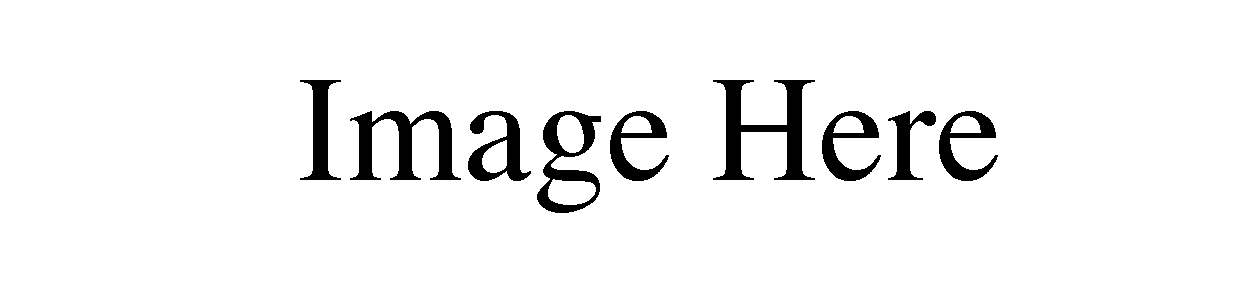
\includegraphics[width=0.6\textwidth]{./img/Dummy.pdf}
	\setlength{\abovecaptionskip}{0cm}
	\caption{Caption For Figure}
	\label{fig: Label For Figure}
\end{figure}

\subsection{Tables}

\begin{table}[!ht]
	\setstretch{1.3}
	\centering
	\begin{tabular}{cc}
		\toprule
		Notation                      & Explanation                                       \\
		\midrule
		$\operatorname{ARIMA}(p,d,q)$ & ARIMA                                             \\
		$p$                           & order of the $\operatorname{AR}$(Auto Regressive) \\
		$d$                           & the number of differences order                   \\
		$q$                           & order of the $\operatorname{MA}$(Moving Average)  \\
		$\phi$                        & $\operatorname{AR}$ Coefficient                   \\
		$\theta$                      & $\operatorname{MA}$ Coefficient                   \\
		$\hat{y}_{t}$                 & the predicted price of gold / bitcoin at time $t$ \\
		\bottomrule
	\end{tabular}
	\caption{Caption For Table}
	\label{tab: Label For Table}
\end{table}

\subsection{Subfigures}

\begin{figure}[!ht]
	\begin{subfigure}[t]{.45\linewidth}
		\centering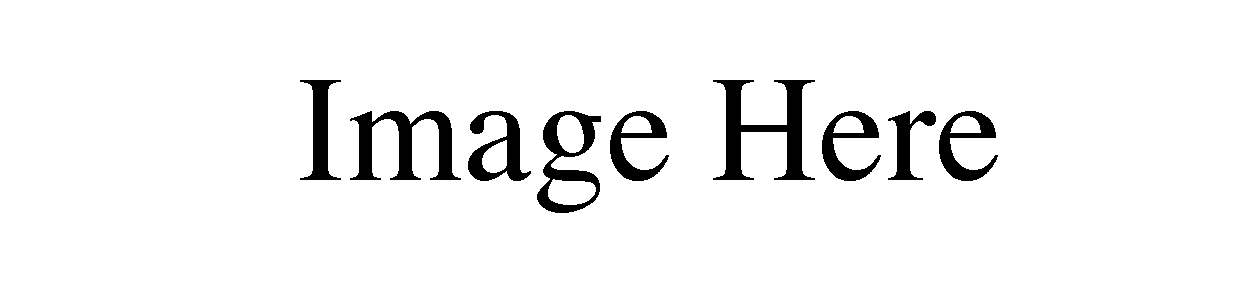
\includegraphics[width=0.9\linewidth]{./img/Dummy.pdf}
		\caption{Caption For Subfigure}
		\label{fig: Label For Subfigure a}
	\end{subfigure}
	\begin{subfigure}[t]{.45\linewidth}
		\centering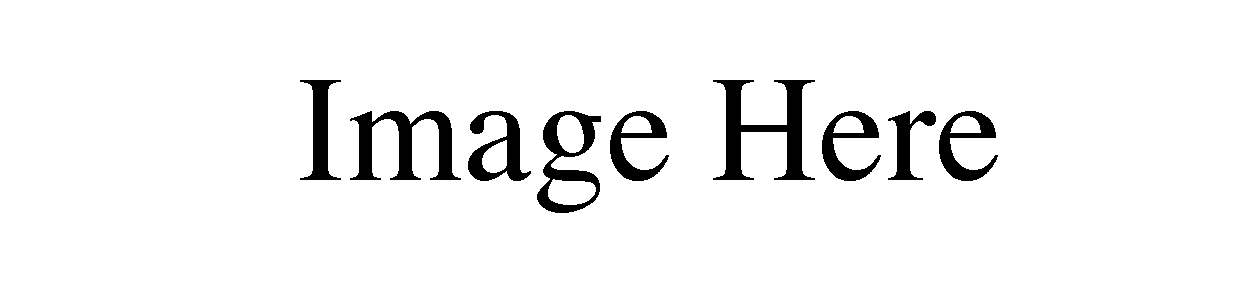
\includegraphics[width=0.9\linewidth]{./img/Dummy.pdf}
		\caption{Caption For Subfigure}
		\label{fig: Label For Subfigure b}
	\end{subfigure}
	\\
	\begin{subfigure}[t]{.45\linewidth}
		\centering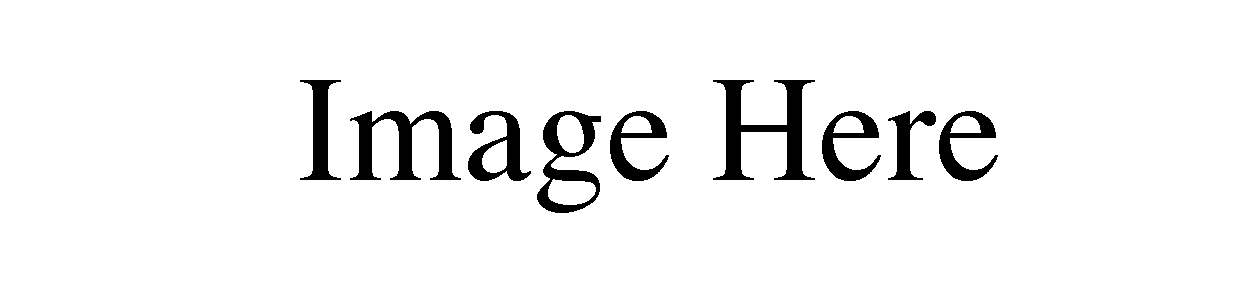
\includegraphics[width=0.9\linewidth]{./img/Dummy.pdf}
		\caption{Caption For Subfigure}
		\label{fig: Label For Subfigure c}
	\end{subfigure}
	\begin{subfigure}[t]{.45\linewidth}
		\centering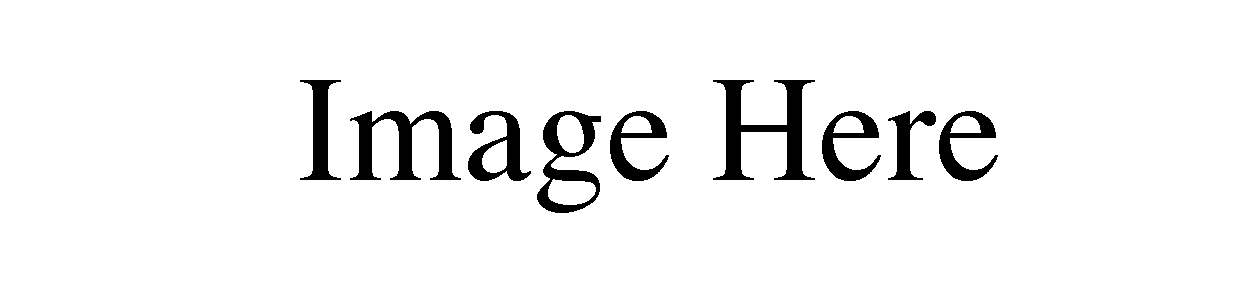
\includegraphics[width=0.9\linewidth]{./img/Dummy.pdf}
		\caption{Caption For Subfigure}
		\label{fig: Label For Subfigure d}
	\end{subfigure}
	\caption{Caption For Main Figure}
	\label{fig: Label For Main Figure}
\end{figure}

% \subsection{Listings}

\lstinputlisting[
	style=ANSI-C,
	label={code: c-mwe},
	caption={C Minimal Working Example},
	linerange={1-3},
]{./source/mwe.c}

\subsection{Symbols}

\begin{table}[!ht]
	\renewcommand{\arraystretch}{2.0}
	\centering
	\begin{tabular}{llll}
		\toprule
		Output                       & Code                                &
		Output                       & Code                                  \\
		\midrule
		\textit{itshape}             & \verb|\textit{itshape}|             &
		\texttt{ttshape}             & \verb|\texttt{ttshape}|               \\
		\textbf{bold}                & \verb|\textbf{bold}|                &
		$\textrm{normal}$            & \verb|$\textrm{normal}$|              \\
		\midrule
		$\{\}$                       & \verb|$\{\}$|                       &
		\$                           & \verb|\$|                             \\
		\%                           & \verb|\%|                           &
		\#                           & \verb|\#|                             \\
		\midrule
		$x^{i}_{j}$                  & \verb|x^{i}_{j}|                    &
		$\dfrac{i}{j}$               & \verb|$\dfrac{i}{j}$|                 \\
		$\hat{p}$                    & \verb|$\hat{p}$|                    &
		$\bar{X}$                    & \verb|$\bar{X}$|                      \\
		$\sum_{i}^{j}$               & \verb|$\sum_{i}^{j}$|               &
		$\displaystyle\sum_{i}^{j}$  & \verb|$\displaystyle\sum_{i}^{j}$|    \\
		$X\overset{ind}{\sim}N(0,1)$ & \verb|$X\overset{ind}{\sim}N(0,1)$| &
		$\left( content \right)$     & \verb|$\left( content \right)$|       \\
		$\geqslant$                  & \verb|$\geqslant$|                  &
		$\leqslant$                  & \verb|$\leqslant$|                    \\
		$\cdots$                     & \verb|$\cdots$|                     &
		$\cdot$                      & \verb|$\cdot$|                        \\
		$\infty$                     & \verb|$\infty$|                     &
		$\nabla$                     & \verb|$\nabla$|                       \\
		$\lceil x \rceil$            & \verb|$\lceil x \rceil$|            &
		$\lfloor x \rfloor$          & \verb|$\lfloor x \rfloor$|            \\
		$\min x$                     & \verb|$\min x$|                     &
		$\max x$                     & \verb|$\max x$|                       \\
		$\log_{a}{b}$                & \verb|$\log_{a}{b}$|                &
		$\lim_{x \to a} $            & \verb|$\lim_{x \to a}$|               \\
		\bottomrule
	\end{tabular}
	\caption{Commonly used \LaTeX \, command}
	\label{tab: commonly used LaTeX command}
\end{table}

\subsection{Environments}

\subsubsection{Lists}
Ordered list
\begin{enumerate}[1)]
	\item item 1
	\item item 2
	      \begin{enumerate}[a)]
		      \item nested item 1
		      \item nested item 2
	      \end{enumerate}
\end{enumerate}

Unordered list
\begin{itemize}
	\item item 1
	\item item 2
	      \begin{itemize}
		      \item nested item 1
		      \item nested item 2
	      \end{itemize}
\end{itemize}

\subsubsection{Math}

\subsubsection{Multiline Formula}
\begin{gather*}
	a + b = c \\
	c + d = e
\end{gather*}

\subsubsection{Matrix}
\[
	\begin{bmatrix}
		a & b & c \\
		d & e & f \\
		g & h & i
	\end{bmatrix}
\]

\subsubsection{System of equations}
\[
	\begin{dcases}
		a + b = c \\
		d + e = f
	\end{dcases}
\]

\section{Self-Define Environments}

\begin{Def}{test}{}
  test
\end{Def}

